\documentclass{beamer}

\usetheme{Boadilla}

\usepackage{times}
\usefonttheme{structurebold}
\usepackage{listings}
\usepackage{listings-rust}

\usepackage{pgf}
\usepackage{tikz}
\usepackage{alltt}
\usepackage[normalem]{ulem}
\usetikzlibrary{arrows,automata,shapes,positioning}
\usepackage{amsmath,amssymb}
\usepackage{rotating}
\usepackage{ulem}
\usepackage{pythonhighlight}
\usepackage{amssymb}
\usepackage{pifont}
\newcommand{\xmark}{\ding{55}}
\usepackage{dafny}

\usetikzlibrary{arrows,automata,shapes}
\tikzstyle{block} = [rectangle, draw, fill=blue!20, 
    text width=5em, text centered, rounded corners, minimum height=2em]
\tikzstyle{bt} = [rectangle, draw, fill=blue!20, 
    text width=4em, text centered, rounded corners, minimum height=2em]

\lstset{ %
language=Rust}

%\setbeamercovered{dynamic}
\setbeamertemplate{footline}[page number]{}
\setbeamertemplate{navigation symbols}{}
\usefonttheme{structurebold}

\title{Software Testing, Quality Assurance \& Maintenance---Lecture 18}
\author{Patrick Lam\\University of Waterloo}
\date{March 13, 2026}

\colorlet{redshaded}{red!25!bg}
\colorlet{shaded}{black!25!bg}
\colorlet{shadedshaded}{black!10!bg}
\colorlet{blackshaded}{black!40!bg}

\colorlet{darkred}{red!80!black}
\colorlet{darkblue}{blue!80!black}
\colorlet{darkgreen}{green!80!black}

\newcommand{\rot}[1]{\rotatebox{90}{\mbox{#1}}}
\newcommand{\gray}[1]{\mbox{#1}}

\newenvironment{changemargin}[1]{% 
  \begin{list}{}{% 
    \setlength{\topsep}{0pt}% 
    \setlength{\leftmargin}{#1}% 
    \setlength{\rightmargin}{1em}
    \setlength{\listparindent}{\parindent}% 
    \setlength{\itemindent}{\parindent}% 
    \setlength{\parsep}{\parskip}% 
  }% 
  \item[]}{\end{list}}

\newcommand{\brac}[1]{\texttt{\textless #1\textgreater}}


\begin{document}
\begin{frame}
  \titlepage
\end{frame}


\usebackgroundtemplate{\tikz\node[opacity=0.3]{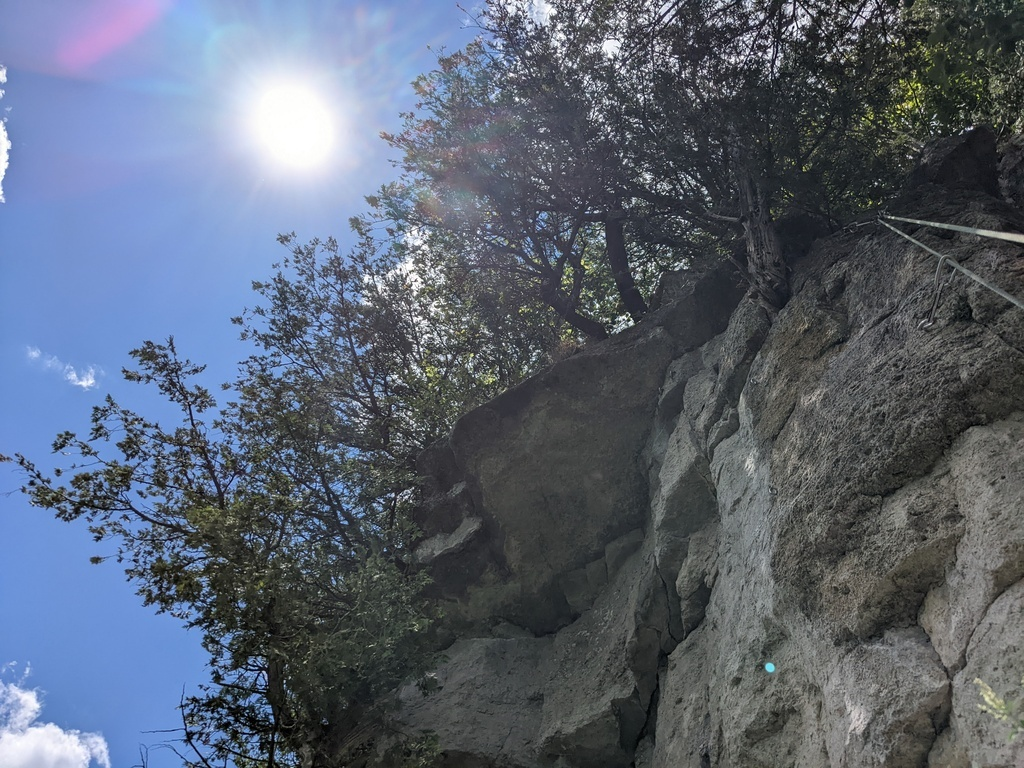
\includegraphics[width=\paperwidth]{L17/PXL_20220729_181423529.jpg}};}
\begin{frame}
  \frametitle{More Dafny Motivation}
  \begin{changemargin}{2cm}
    {    \Large
      Last time: talked about verifying Cedar (authorization library).\\[1em]
      
      Dafny proves user-specified annotations and verifies absence of runtime errors.\\[1em]
      Runtime errors: usually undefined behaviour at best, e.g. out-of-bounds array accesses, null dereferences, etc.\\[1em]

      Alternative option: symbolic execution and bounded model checking. But Dafny is fully-static, and aims to work on real code.
}
  \end{changemargin}
\end{frame}
\usebackgroundtemplate{}

\begin{frame}
  \frametitle{Other Verified Software}
  \begin{changemargin}{1cm}
        \large
\begin{itemize}
\item Paris Metro line 14 control system (B): 110,000 lines of models, 86,000 lines of Ada.
\item seL4 (Haskell, Isabelle/HOL, C): conforms to its specification and maintains integrity and confidentiality.
\item CompCert (Coq): a formally verified optimizing compiler
\item IronClad (Dafny): establishes guarantees about how remote apps behave
\end{itemize}

First 3 by verification experts; IronClad by systems programmers.\\[1em]
All of these projects verified from the start.\\[1em]
More about formal verification \& software development afterwards.
  \end{changemargin}
\end{frame}

\begin{frame}
  \frametitle{Dafny Examples}
    \Large
  \begin{changemargin}{2cm}
    No slides; we'll work through\\
  \end{changemargin}
\large
\begin{center}  \url{https://dafny.org/dafny/OnlineTutorial/guide}
\end{center}
\end{frame}
    

\end{document}
